
% Default to the notebook output style

    


% Inherit from the specified cell style.




    
\documentclass[11pt]{article}

    
    
    \usepackage[T1]{fontenc}
    % Nicer default font (+ math font) than Computer Modern for most use cases
    \usepackage{mathpazo}

    % Basic figure setup, for now with no caption control since it's done
    % automatically by Pandoc (which extracts ![](path) syntax from Markdown).
    \usepackage{graphicx}
    % We will generate all images so they have a width \maxwidth. This means
    % that they will get their normal width if they fit onto the page, but
    % are scaled down if they would overflow the margins.
    \makeatletter
    \def\maxwidth{\ifdim\Gin@nat@width>\linewidth\linewidth
    \else\Gin@nat@width\fi}
    \makeatother
    \let\Oldincludegraphics\includegraphics
    % Set max figure width to be 80% of text width, for now hardcoded.
    \renewcommand{\includegraphics}[1]{\Oldincludegraphics[width=.9\maxwidth]{#1}}
    % Ensure that by default, figures have no caption (until we provide a
    % proper Figure object with a Caption API and a way to capture that
    % in the conversion process - todo).
    \usepackage{caption}
    \DeclareCaptionLabelFormat{nolabel}{}
    \captionsetup{labelformat=nolabel}

    \usepackage{adjustbox} % Used to constrain images to a maximum size 
    \usepackage{framed}
    \usepackage{xcolor} % Allow colors to be defined
    \usepackage{enumerate} % Needed for markdown enumerations to work
    \usepackage{geometry} % Used to adjust the document margins
    \usepackage{amsmath} % Equations
    \usepackage{amssymb} % Equations
    \usepackage{textcomp} % defines textquotesingle
    % Hack from http://tex.stackexchange.com/a/47451/13684:
    \AtBeginDocument{%
        \def\PYZsq{\textquotesingle}% Upright quotes in Pygmentized code
    }
    \usepackage{upquote} % Upright quotes for verbatim code
    \usepackage{eurosym} % defines \euro
    \usepackage[mathletters]{ucs} % Extended unicode (utf-8) support
    \usepackage[utf8x]{inputenc} % Allow utf-8 characters in the tex document
    \usepackage{fancyvrb} % verbatim replacement that allows latex
    \usepackage{grffile} % extends the file name processing of package graphics 
                         % to support a larger range 
    % The hyperref package gives us a pdf with properly built
    % internal navigation ('pdf bookmarks' for the table of contents,
    % internal cross-reference links, web links for URLs, etc.)
    \usepackage{hyperref}
    \usepackage{longtable} % longtable support required by pandoc >1.10
    \usepackage{booktabs}  % table support for pandoc > 1.12.2
    \usepackage[inline]{enumitem} % IRkernel/repr support (it uses the enumerate* environment)
    \usepackage[normalem]{ulem} % ulem is needed to support strikethroughs (\sout)
                                % normalem makes italics be italics, not underlines
    

    
    
    % Colors for the hyperref package
    \definecolor{urlcolor}{rgb}{0,.145,.698}
    \definecolor{linkcolor}{rgb}{.71,0.21,0.01}
    \definecolor{citecolor}{rgb}{.12,.54,.11}

    % ANSI colors
    \definecolor{ansi-black}{HTML}{3E424D}
    \definecolor{ansi-black-intense}{HTML}{282C36}
    \definecolor{ansi-red}{HTML}{E75C58}
    \definecolor{ansi-red-intense}{HTML}{B22B31}
    \definecolor{ansi-green}{HTML}{00A250}
    \definecolor{ansi-green-intense}{HTML}{007427}
    \definecolor{ansi-yellow}{HTML}{DDB62B}
    \definecolor{ansi-yellow-intense}{HTML}{B27D12}
    \definecolor{ansi-blue}{HTML}{208FFB}
    \definecolor{ansi-blue-intense}{HTML}{0065CA}
    \definecolor{ansi-magenta}{HTML}{D160C4}
    \definecolor{ansi-magenta-intense}{HTML}{A03196}
    \definecolor{ansi-cyan}{HTML}{60C6C8}
    \definecolor{ansi-cyan-intense}{HTML}{258F8F}
    \definecolor{ansi-white}{HTML}{C5C1B4}
    \definecolor{ansi-white-intense}{HTML}{A1A6B2}
	\definecolor{shadecolor}{HTML}{E3E3E3}

    % commands and environments needed by pandoc snippets
    % extracted from the output of `pandoc -s`
    \providecommand{\tightlist}{%
      \setlength{\itemsep}{0pt}\setlength{\parskip}{0pt}}
    \DefineVerbatimEnvironment{Highlighting}{Verbatim}{commandchars=\\\{\}}
    % Add ',fontsize=\small' for more characters per line
    \newenvironment{Shaded}{}{}
    \newcommand{\KeywordTok}[1]{\textcolor[rgb]{0.00,0.44,0.13}{\textbf{{#1}}}}
    \newcommand{\DataTypeTok}[1]{\textcolor[rgb]{0.56,0.13,0.00}{{#1}}}
    \newcommand{\DecValTok}[1]{\textcolor[rgb]{0.25,0.63,0.44}{{#1}}}
    \newcommand{\BaseNTok}[1]{\textcolor[rgb]{0.25,0.63,0.44}{{#1}}}
    \newcommand{\FloatTok}[1]{\textcolor[rgb]{0.25,0.63,0.44}{{#1}}}
    \newcommand{\CharTok}[1]{\textcolor[rgb]{0.25,0.44,0.63}{{#1}}}
    \newcommand{\StringTok}[1]{\textcolor[rgb]{0.25,0.44,0.63}{{#1}}}
    \newcommand{\CommentTok}[1]{\textcolor[rgb]{0.38,0.63,0.69}{\textit{{#1}}}}
    \newcommand{\OtherTok}[1]{\textcolor[rgb]{0.00,0.44,0.13}{{#1}}}
    \newcommand{\AlertTok}[1]{\textcolor[rgb]{1.00,0.00,0.00}{\textbf{{#1}}}}
    \newcommand{\FunctionTok}[1]{\textcolor[rgb]{0.02,0.16,0.49}{{#1}}}
    \newcommand{\RegionMarkerTok}[1]{{#1}}
    \newcommand{\ErrorTok}[1]{\textcolor[rgb]{1.00,0.00,0.00}{\textbf{{#1}}}}
    \newcommand{\NormalTok}[1]{{#1}}
    
    % Additional commands for more recent versions of Pandoc
    \newcommand{\ConstantTok}[1]{\textcolor[rgb]{0.53,0.00,0.00}{{#1}}}
    \newcommand{\SpecialCharTok}[1]{\textcolor[rgb]{0.25,0.44,0.63}{{#1}}}
    \newcommand{\VerbatimStringTok}[1]{\textcolor[rgb]{0.25,0.44,0.63}{{#1}}}
    \newcommand{\SpecialStringTok}[1]{\textcolor[rgb]{0.73,0.40,0.53}{{#1}}}
    \newcommand{\ImportTok}[1]{{#1}}
    \newcommand{\DocumentationTok}[1]{\textcolor[rgb]{0.73,0.13,0.13}{\textit{{#1}}}}
    \newcommand{\AnnotationTok}[1]{\textcolor[rgb]{0.38,0.63,0.69}{\textbf{\textit{{#1}}}}}
    \newcommand{\CommentVarTok}[1]{\textcolor[rgb]{0.38,0.63,0.69}{\textbf{\textit{{#1}}}}}
    \newcommand{\VariableTok}[1]{\textcolor[rgb]{0.10,0.09,0.49}{{#1}}}
    \newcommand{\ControlFlowTok}[1]{\textcolor[rgb]{0.00,0.44,0.13}{\textbf{{#1}}}}
    \newcommand{\OperatorTok}[1]{\textcolor[rgb]{0.40,0.40,0.40}{{#1}}}
    \newcommand{\BuiltInTok}[1]{{#1}}
    \newcommand{\ExtensionTok}[1]{{#1}}
    \newcommand{\PreprocessorTok}[1]{\textcolor[rgb]{0.74,0.48,0.00}{{#1}}}
    \newcommand{\AttributeTok}[1]{\textcolor[rgb]{0.49,0.56,0.16}{{#1}}}
    \newcommand{\InformationTok}[1]{\textcolor[rgb]{0.38,0.63,0.69}{\textbf{\textit{{#1}}}}}
    \newcommand{\WarningTok}[1]{\textcolor[rgb]{0.38,0.63,0.69}{\textbf{\textit{{#1}}}}}
    
    
    % Define a nice break command that doesn't care if a line doesn't already
    % exist.
    \def\br{\hspace*{\fill} \\* }
    % Math Jax compatability definitions
    \def\gt{>}
    \def\lt{<}
    % Document parameters
    \title{A Solution To The Developer Allocation Problem Using Simulated Annealing}
    
    
    

    % Pygments definitions
    
\makeatletter
\def\PY@reset{\let\PY@it=\relax \let\PY@bf=\relax%
    \let\PY@ul=\relax \let\PY@tc=\relax%
    \let\PY@bc=\relax \let\PY@ff=\relax}
\def\PY@tok#1{\csname PY@tok@#1\endcsname}
\def\PY@toks#1+{\ifx\relax#1\empty\else%
    \PY@tok{#1}\expandafter\PY@toks\fi}
\def\PY@do#1{\PY@bc{\PY@tc{\PY@ul{%
    \PY@it{\PY@bf{\PY@ff{#1}}}}}}}
\def\PY#1#2{\PY@reset\PY@toks#1+\relax+\PY@do{#2}}

\expandafter\def\csname PY@tok@w\endcsname{\def\PY@tc##1{\textcolor[rgb]{0.73,0.73,0.73}{##1}}}
\expandafter\def\csname PY@tok@c\endcsname{\let\PY@it=\textit\def\PY@tc##1{\textcolor[rgb]{0.25,0.50,0.50}{##1}}}
\expandafter\def\csname PY@tok@cp\endcsname{\def\PY@tc##1{\textcolor[rgb]{0.74,0.48,0.00}{##1}}}
\expandafter\def\csname PY@tok@k\endcsname{\let\PY@bf=\textbf\def\PY@tc##1{\textcolor[rgb]{0.00,0.50,0.00}{##1}}}
\expandafter\def\csname PY@tok@kp\endcsname{\def\PY@tc##1{\textcolor[rgb]{0.00,0.50,0.00}{##1}}}
\expandafter\def\csname PY@tok@kt\endcsname{\def\PY@tc##1{\textcolor[rgb]{0.69,0.00,0.25}{##1}}}
\expandafter\def\csname PY@tok@o\endcsname{\def\PY@tc##1{\textcolor[rgb]{0.40,0.40,0.40}{##1}}}
\expandafter\def\csname PY@tok@ow\endcsname{\let\PY@bf=\textbf\def\PY@tc##1{\textcolor[rgb]{0.67,0.13,1.00}{##1}}}
\expandafter\def\csname PY@tok@nb\endcsname{\def\PY@tc##1{\textcolor[rgb]{0.00,0.50,0.00}{##1}}}
\expandafter\def\csname PY@tok@nf\endcsname{\def\PY@tc##1{\textcolor[rgb]{0.00,0.00,1.00}{##1}}}
\expandafter\def\csname PY@tok@nc\endcsname{\let\PY@bf=\textbf\def\PY@tc##1{\textcolor[rgb]{0.00,0.00,1.00}{##1}}}
\expandafter\def\csname PY@tok@nn\endcsname{\let\PY@bf=\textbf\def\PY@tc##1{\textcolor[rgb]{0.00,0.00,1.00}{##1}}}
\expandafter\def\csname PY@tok@ne\endcsname{\let\PY@bf=\textbf\def\PY@tc##1{\textcolor[rgb]{0.82,0.25,0.23}{##1}}}
\expandafter\def\csname PY@tok@nv\endcsname{\def\PY@tc##1{\textcolor[rgb]{0.10,0.09,0.49}{##1}}}
\expandafter\def\csname PY@tok@no\endcsname{\def\PY@tc##1{\textcolor[rgb]{0.53,0.00,0.00}{##1}}}
\expandafter\def\csname PY@tok@nl\endcsname{\def\PY@tc##1{\textcolor[rgb]{0.63,0.63,0.00}{##1}}}
\expandafter\def\csname PY@tok@ni\endcsname{\let\PY@bf=\textbf\def\PY@tc##1{\textcolor[rgb]{0.60,0.60,0.60}{##1}}}
\expandafter\def\csname PY@tok@na\endcsname{\def\PY@tc##1{\textcolor[rgb]{0.49,0.56,0.16}{##1}}}
\expandafter\def\csname PY@tok@nt\endcsname{\let\PY@bf=\textbf\def\PY@tc##1{\textcolor[rgb]{0.00,0.50,0.00}{##1}}}
\expandafter\def\csname PY@tok@nd\endcsname{\def\PY@tc##1{\textcolor[rgb]{0.67,0.13,1.00}{##1}}}
\expandafter\def\csname PY@tok@s\endcsname{\def\PY@tc##1{\textcolor[rgb]{0.73,0.13,0.13}{##1}}}
\expandafter\def\csname PY@tok@sd\endcsname{\let\PY@it=\textit\def\PY@tc##1{\textcolor[rgb]{0.73,0.13,0.13}{##1}}}
\expandafter\def\csname PY@tok@si\endcsname{\let\PY@bf=\textbf\def\PY@tc##1{\textcolor[rgb]{0.73,0.40,0.53}{##1}}}
\expandafter\def\csname PY@tok@se\endcsname{\let\PY@bf=\textbf\def\PY@tc##1{\textcolor[rgb]{0.73,0.40,0.13}{##1}}}
\expandafter\def\csname PY@tok@sr\endcsname{\def\PY@tc##1{\textcolor[rgb]{0.73,0.40,0.53}{##1}}}
\expandafter\def\csname PY@tok@ss\endcsname{\def\PY@tc##1{\textcolor[rgb]{0.10,0.09,0.49}{##1}}}
\expandafter\def\csname PY@tok@sx\endcsname{\def\PY@tc##1{\textcolor[rgb]{0.00,0.50,0.00}{##1}}}
\expandafter\def\csname PY@tok@m\endcsname{\def\PY@tc##1{\textcolor[rgb]{0.40,0.40,0.40}{##1}}}
\expandafter\def\csname PY@tok@gh\endcsname{\let\PY@bf=\textbf\def\PY@tc##1{\textcolor[rgb]{0.00,0.00,0.50}{##1}}}
\expandafter\def\csname PY@tok@gu\endcsname{\let\PY@bf=\textbf\def\PY@tc##1{\textcolor[rgb]{0.50,0.00,0.50}{##1}}}
\expandafter\def\csname PY@tok@gd\endcsname{\def\PY@tc##1{\textcolor[rgb]{0.63,0.00,0.00}{##1}}}
\expandafter\def\csname PY@tok@gi\endcsname{\def\PY@tc##1{\textcolor[rgb]{0.00,0.63,0.00}{##1}}}
\expandafter\def\csname PY@tok@gr\endcsname{\def\PY@tc##1{\textcolor[rgb]{1.00,0.00,0.00}{##1}}}
\expandafter\def\csname PY@tok@ge\endcsname{\let\PY@it=\textit}
\expandafter\def\csname PY@tok@gs\endcsname{\let\PY@bf=\textbf}
\expandafter\def\csname PY@tok@gp\endcsname{\let\PY@bf=\textbf\def\PY@tc##1{\textcolor[rgb]{0.00,0.00,0.50}{##1}}}
\expandafter\def\csname PY@tok@go\endcsname{\def\PY@tc##1{\textcolor[rgb]{0.53,0.53,0.53}{##1}}}
\expandafter\def\csname PY@tok@gt\endcsname{\def\PY@tc##1{\textcolor[rgb]{0.00,0.27,0.87}{##1}}}
\expandafter\def\csname PY@tok@err\endcsname{\def\PY@bc##1{\setlength{\fboxsep}{0pt}\fcolorbox[rgb]{1.00,0.00,0.00}{1,1,1}{\strut ##1}}}
\expandafter\def\csname PY@tok@kc\endcsname{\let\PY@bf=\textbf\def\PY@tc##1{\textcolor[rgb]{0.00,0.50,0.00}{##1}}}
\expandafter\def\csname PY@tok@kd\endcsname{\let\PY@bf=\textbf\def\PY@tc##1{\textcolor[rgb]{0.00,0.50,0.00}{##1}}}
\expandafter\def\csname PY@tok@kn\endcsname{\let\PY@bf=\textbf\def\PY@tc##1{\textcolor[rgb]{0.00,0.50,0.00}{##1}}}
\expandafter\def\csname PY@tok@kr\endcsname{\let\PY@bf=\textbf\def\PY@tc##1{\textcolor[rgb]{0.00,0.50,0.00}{##1}}}
\expandafter\def\csname PY@tok@bp\endcsname{\def\PY@tc##1{\textcolor[rgb]{0.00,0.50,0.00}{##1}}}
\expandafter\def\csname PY@tok@fm\endcsname{\def\PY@tc##1{\textcolor[rgb]{0.00,0.00,1.00}{##1}}}
\expandafter\def\csname PY@tok@vc\endcsname{\def\PY@tc##1{\textcolor[rgb]{0.10,0.09,0.49}{##1}}}
\expandafter\def\csname PY@tok@vg\endcsname{\def\PY@tc##1{\textcolor[rgb]{0.10,0.09,0.49}{##1}}}
\expandafter\def\csname PY@tok@vi\endcsname{\def\PY@tc##1{\textcolor[rgb]{0.10,0.09,0.49}{##1}}}
\expandafter\def\csname PY@tok@vm\endcsname{\def\PY@tc##1{\textcolor[rgb]{0.10,0.09,0.49}{##1}}}
\expandafter\def\csname PY@tok@sa\endcsname{\def\PY@tc##1{\textcolor[rgb]{0.73,0.13,0.13}{##1}}}
\expandafter\def\csname PY@tok@sb\endcsname{\def\PY@tc##1{\textcolor[rgb]{0.73,0.13,0.13}{##1}}}
\expandafter\def\csname PY@tok@sc\endcsname{\def\PY@tc##1{\textcolor[rgb]{0.73,0.13,0.13}{##1}}}
\expandafter\def\csname PY@tok@dl\endcsname{\def\PY@tc##1{\textcolor[rgb]{0.73,0.13,0.13}{##1}}}
\expandafter\def\csname PY@tok@s2\endcsname{\def\PY@tc##1{\textcolor[rgb]{0.73,0.13,0.13}{##1}}}
\expandafter\def\csname PY@tok@sh\endcsname{\def\PY@tc##1{\textcolor[rgb]{0.73,0.13,0.13}{##1}}}
\expandafter\def\csname PY@tok@s1\endcsname{\def\PY@tc##1{\textcolor[rgb]{0.73,0.13,0.13}{##1}}}
\expandafter\def\csname PY@tok@mb\endcsname{\def\PY@tc##1{\textcolor[rgb]{0.40,0.40,0.40}{##1}}}
\expandafter\def\csname PY@tok@mf\endcsname{\def\PY@tc##1{\textcolor[rgb]{0.40,0.40,0.40}{##1}}}
\expandafter\def\csname PY@tok@mh\endcsname{\def\PY@tc##1{\textcolor[rgb]{0.40,0.40,0.40}{##1}}}
\expandafter\def\csname PY@tok@mi\endcsname{\def\PY@tc##1{\textcolor[rgb]{0.40,0.40,0.40}{##1}}}
\expandafter\def\csname PY@tok@il\endcsname{\def\PY@tc##1{\textcolor[rgb]{0.40,0.40,0.40}{##1}}}
\expandafter\def\csname PY@tok@mo\endcsname{\def\PY@tc##1{\textcolor[rgb]{0.40,0.40,0.40}{##1}}}
\expandafter\def\csname PY@tok@ch\endcsname{\let\PY@it=\textit\def\PY@tc##1{\textcolor[rgb]{0.25,0.50,0.50}{##1}}}
\expandafter\def\csname PY@tok@cm\endcsname{\let\PY@it=\textit\def\PY@tc##1{\textcolor[rgb]{0.25,0.50,0.50}{##1}}}
\expandafter\def\csname PY@tok@cpf\endcsname{\let\PY@it=\textit\def\PY@tc##1{\textcolor[rgb]{0.25,0.50,0.50}{##1}}}
\expandafter\def\csname PY@tok@c1\endcsname{\let\PY@it=\textit\def\PY@tc##1{\textcolor[rgb]{0.25,0.50,0.50}{##1}}}
\expandafter\def\csname PY@tok@cs\endcsname{\let\PY@it=\textit\def\PY@tc##1{\textcolor[rgb]{0.25,0.50,0.50}{##1}}}

\def\PYZbs{\char`\\}
\def\PYZus{\char`\_}
\def\PYZob{\char`\{}
\def\PYZcb{\char`\}}
\def\PYZca{\char`\^}
\def\PYZam{\char`\&}
\def\PYZlt{\char`\<}
\def\PYZgt{\char`\>}
\def\PYZsh{\char`\#}
\def\PYZpc{\char`\%}
\def\PYZdl{\char`\$}
\def\PYZhy{\char`\-}
\def\PYZsq{\char`\'}
\def\PYZdq{\char`\"}
\def\PYZti{\char`\~}
% for compatibility with earlier versions
\def\PYZat{@}
\def\PYZlb{[}
\def\PYZrb{]}
\makeatother


    % Exact colors from NB
    \definecolor{incolor}{rgb}{0.0, 0.0, 0.5}
    \definecolor{outcolor}{rgb}{0.545, 0.0, 0.0}



    
    % Prevent overflowing lines due to hard-to-break entities
    \sloppy 
    % Setup hyperref package
    \hypersetup{
      breaklinks=true,  % so long urls are correctly broken across lines
      colorlinks=true,
      urlcolor=urlcolor,
      linkcolor=linkcolor,
      citecolor=citecolor,
      }
    % Slightly bigger margins than the latex defaults
    
    \geometry{verbose,tmargin=1in,bmargin=1in,lmargin=.5in,rmargin=.5in}
    
    \author{Jorge Reyes-Spindola}

    \begin{document}
        
    \maketitle
       
\section{Introduction}\label{introduction}

At large companies the project-developer allocation problem is
encountered all the time. There are a number of projects available and
requiring resources and developers wishing to work on them. The projects
are managed by one or more project managers (PMs) and developers are
required to rank a certain number of projects in order of preference.
This process is the one-sided variant of the problem. The two-sided
would be when the project (or PM) expresses preference for a programmer
or programmers.

Usually, only one developer or pair of developers work on a given
project. The problem arises when several developers choose a particular
project as their first choice. Inevitably, some developers will be
assigned their second or third choices which in turn causes secondary
effects because the less preferred projects could be the first choice of
another developer.

An additional issue is the PM's workload. Usually, a PM will propose
more projects than they can feasibly oversee in order to provide a wider
range of developer choices. Further complications arise when all of a
PM's projects are popular because it guarantees some developers will not
be assigned their first choice.

The developer-project problem is a specific case of the generalized
assignment problem, a well-known optimization problem that consists of
assigning sets of jobs to sets of agents while minimizing the cost
associated with the assignment; this problem can be formulated as an
integer linear problem. A wide range of methods have been devised for
solving such problems including, a genetic algorithm, and a local-ratio
technique for the knapsack problem.

In this paper we investigate how simulated annealing (SA), a method from
statistical and computational physics, can be used to obtain a "good
enough" solution to the developer-project problem.

    \section{Problem Specification}\label{problem-specification}

We focus on the assignment of development projects at an unnamed
company. Each developer (or team of developers) is invited to submit a
list of four project preferences, ranking them from 1 to 4 in order of
preference (1 = most preferred). The PMs then assign developers to
projects with the goal of maximizing developer satisfaction while
meeting the following constraints: 

\begin{enumerate}
\def\labelenumi{\arabic{enumi}.}
\tightlist
\item
Each developer is assigned to one
of the projects on their preference list.
\item
No project can be assigned
to more than one developer (or team of developers). 
\item 
PMs cannot be
assigned more projects than they can feasibly oversee.
\end{enumerate}

The mathematical framing of the problem is as follows:

Let \(N\) be the number of developers, \(M\) is the number of projects
(with \(M \gt N\)) and \(S\) is the number of PMs. Define a
\(N \times M\) matrix \(C\) with elements


\begin{equation}\label{E:first}
C_{ij} = \begin{cases}
1 & \text{if developer $i$ chose project $j$} \\ 
0 & \text{otherwise}, 
\end{cases}.
\end{equation}


and define an \(N \times M\) allocation matrix \(X\) by

\begin{equation}\label{E:allocation}
X_{ij} =  \begin{cases}
1 & \text{if developer $i$ is assigned to project $j$} \\ 
0 & \text{otherwise.}
\end{cases}
\end{equation}


Our goal is to maximize developer satisfaction. To do so, we need a
definition of satisfaction. Clearly, developers will be happier if they
receive their first choice and less happy if they receive their fourth
choice. We define 

\begin{equation}\label{objective}
\mathfrak O = \sum_{k=1}^4 w_k n_k
\end{equation}

where \(n_k\) is the number of developers assigned their \(k\)th
choice in the allocation and \(w_k\) is the weighting assigned to the
\(k\)th choice, with \(w_k \gt w_{k+1}\). The sum in equation
(\ref{objective}) is our measure of overall satisfaction. In the
optimization literature such a quantity is referred to as the
\emph{objective function}.

The first two constraints can be written simply as

\begin{align}
\sum_{j=1}^M C_{ij}X_{ij} &= 1 \;\;\; \forall i = 1, \ldots, N \label{const1}\\
\sum_{i=1}^N X_{ij} &\leq 1 \;\;\; \forall j=1, \ldots, M. \label{const2}
\end{align}


To incorporate the third constraint, we let \(F_s\) denote the number of
projects that supervisor \(s\) has in the assignment, and \(L_s\) denote
the largest number of projects they can oversee. Then

\begin{equation}
F_s \leq L_s \;\;\; \forall s = 1, \ldots, S. \label{const3}
\end{equation}

Given a matrix of choices \(C\), our goal is to find an allocation
\(X_{ij}\) that maximizes the value of \(\mathfrak O\) given the weights
\(w_k\) and the constraints in equations (\ref{const1}) - (\ref{const3}). 
The following section will describe the SA algorithm that is used to solve this problem.

    \section{Simulated Annealing}\label{simulated-annealing}

Annealing is the physical process of heating up a solid until it melts,
followed by cooling it down until crystallizes into a state with a
perfect lattice. During this process, the free energy of the solid is
minimized. Practice has shown that the cooling must be done carefully in
order not to get trapped in locally optimal lattice structures with
crystal imperfections.

In combinatorial optimization, we can define a similar process. This
process can be formulated as the problem of finding -among a potentially
very large number of solutions- a solution with minimal cost. Now, by
establishing a correspondence between the cost of functions and the free
energy, and between the solutions and the physical states, we can
introduce a solution method in the field of combinatorial optimization
based on a simulation of the physical annealing process. The resulting
method is called \emph{Simulated Annealing}.

Salient features of this method are its general applicability and its
ability to obtain solutions arbitrarily close to an optimum. A major
drawback however, is that finding high-quality solutions may require
large computational efforts.

\subsection{The Metropolis Algorithm}\label{the-metropolis-algorithm}

The physical annealing process can be modelled successfully by using
computer simulation methods from condensed matter physics. As far back
as 1953, Metropolis, \emph{et.al.} introduced a simple algorithm for
simulation the evolution of a solid in a heat bath to \emph{thermal
equilibrium}. The algorithm introduced is based on \emph{Monte Carlo
techniques} and generates a sequence of states of the solid in the
following way. Given a current state \(i\) of the solid with energy
\(E_i\), then a subsequent state \(j\) is generated by applying a
perturbation mechanism which transforms the current state into a next
state by a small distortion, for instance by displacement of a particle.
The energy of the next state is \(E_j\). If \emph{energy difference}
\(E_j - E_i\) is less than or equal to 0, the state \(j\) is accepted as
the current state. If the energy difference is greater than 0, the state
\(j\) is accepted with a certain probability given by


\begin{equation}
\exp \left(  \dfrac{E_i-E_j}{k_B T} \right)
\end{equation}


where \(T\) denotes the \emph{temperature} of the heat bath and \(k_B\)
a physical constant known as the \emph{Boltzmann constant}. The
acceptance rule described above is known as the \emph{Metropolis
criterion} and the algorithm that goes with it is known as the
\emph{Metropolis algorithm}.

\subsection{The SA Algorithm}\label{the-sa-algorithm}

Returning to the algorithm, we can apply the Metropolis algorithm to
generate a sequence of solutions of a combinatorial optimization
problem. For this purpose we assume an analogy between a physical
many-particle system and a combinatorial optimization problem based on
the following equivalences.

\begin{itemize}
\tightlist
\item
  Solutions in a combinatorial optimization problem are equivalent to
  states of a physical system.
\item
  The cost of a solution is equivalent to the energy of a state.
\end{itemize}

The simulated annealing algorithm can now be viewed as an iteration of
Metropolis algorithms, evaluated at decreasing values of a control
parameter which plays the role of the temperature. This parameter is
called the \emph{control parameter}. We now introduce the following
definitions.

\textbf{Definition.} Let \((S,f)\) denote an instance of a combinatorial
optimization problem and \(i\) and \(j\) two solutions with cost
\(f(i)\) and \(f(j)\) respectively. Then the \emph{acceptance criterion}
determines whether \(j\) is accepted from \(i\) by applying the
following \emph{acceptance probability}:


\begin{equation}
P_c(\text{accept $j$}) = \begin{cases}
1 & \text{if}\; f(j) \leq f(i) \\
\exp\left(\dfrac{f(i)-f(j)}{c}\right) & \text{if}\; f(j) \gt f(i),
\end{cases}
\end{equation}


where \(c \in \mathbb{R}^+\) denotes the control parameter.

\textbf{Definition.} A \emph{transition} is a combined action resulting
in the transformation of a current solution into a subsequent one. The
action consists of the following two steps: (\emph{i}) application of
the generation mechanism, (\emph{ii}) application of the acceptance
criterion. Therefore, the Metropolis algorithm operates as follows

\begin{enumerate}
\def\labelenumi{\arabic{enumi}.}
\tightlist
\item
  Choose an initial arrangement \(\mathbf{a}\).
\item
  Choose a trial arrangement \(\mathbf{a^\prime}\).
\item
  Calculate the energy difference.
\item
  Generate a random number \(r \in (0,1)\).
\item
  If \(r \lt P(\mathbf{a} \to \mathbf{a^\prime})\), move to state
  \(\mathbf{a^\prime}\)
\item
  Generate a new trial arrangement and return to step 3.
\end{enumerate}

    \section{Implementation}\label{implementation}

To find a good solution of the developer-project allocation problem
using the SA algorithm, we implemented Python code in the following
notebook. The notebook is available in Github (insert link here). While
we won't discuss all the details of the implementation, we will cover
some salient points.

\subsection{Objective function}\label{objective-function}

We strove to maximize developer happiness and so we defined the energy
in terms of the objective function as

\[
E = -\mathfrak{O} = -w_1n_1 -w_2n_2 -w_3n_3 -w_4n_4.
\]

Recall that \(w_k\) is the weight of preference \(k\) and \(n_k\) is the
number of developers assigned their \(k\)th preference. Naturally, the
preference ranking (weights) should decrease with \(k\). We initally
chose to work with a set of linearly decreasing weights, that led to the
objective function

\[
E = -4n_1 -3n_2 - 2n_3 -n_4.
\]

However, after some work, it was observed that this objective function
let to several degenerate (\emph{i.e.} same energy) solutions. Because
we wanted to discriminate among these and because a better way of
gauging developer satisfaction was needed, a new objective function
based on developer's opinions was developed. Developers were polled to
determine their satisfaction outcome on the basis of their project
assignation. Using this data, the new opinion-based weights were now
determined to be \(w_1=4.7\), \(w_2=4.15\), \(w_3=3.0\), and
\(w_4=2.35\), thus obtaining the new normalized objective function

\[
E^\prime = -\dfrac{100}{N}\left[ n_1 + \dfrac{4.15}{4.7}n_2 + \dfrac{3.0}{4.7}n_3 + \dfrac{2.35}{4.7}n_4 \right].
\]

Using this objective function, the energy corresponding to the best
possible allocation has a value of \(E^* = -100\). The best possible
allocation is where every developer gets their first choice project.

\subsection{Sampling Strategy}\label{sampling-strategy}

The starting point for an SA optimization must be an initial allocation
that satisfies the constraints in the equations above. To obtain a
suitable initialization, we randomly assign each developer one of their
four choices. In general, this assignment will lead to multiple
constraint violations with different developers being assigned the same
project and PMs getting overworked. To correct these violations, we
perform a preliminary Monte Carlo procedure in which we choose a
developer at random and randomly re-allocate them to one of their four
project choices. If this proposed change results in a reduction in the
number of violated constraints, we accept the move, otherwise we reject
it. This process is iterated until we obtain an allocation with no
violations, which we take as the initial configuration for the
application of the SA algorithm.

An important aspect of the SA procedure is the manner in which trial
allocations are proposed within the process. The method adopted should
be reversible and ergodic -all allocations should be reachable within
the sampling procedure. These conditions can be achieved by iterating
the following procedure:

\begin{enumerate}
\def\labelenumi{\arabic{enumi}.}
\tightlist
\item
  Choose a developer at random.
\item
  Choose a random integer from 1 to 4.
\item
  If the developer is currently assigned the project corresponding to
  that choice, repeat step 2. Otherwise, assign the developer the trial
  project corresponding to the random choice. This assignment is the
  trial allocation.
\item
  Check that for the trial allocation no project is assigned to multiple
  developers. If a conflict has arisen, retain the current allocation
  and go to step 1.
\item
  Check that the PM workload limit is not violated. If it is, then
  retain the current allocation and go to step 1.
\item
  Calculate the Metropolis acceptance probability
  \(P(\mathbf{a} \to \mathbf{a^\prime})\). Generate a random number
  \(r \in (0,1)\). If \(P \lt r\), retain the current allocation and go
  to step 1. If \(P \geq r\), accept the trial allocation as the current
  allocation.
\end{enumerate}

    \section{Results}\label{results}

A run of initial results is shown here below the notebook. The dataset
used contained 19 developers looking to be allocated amongst 58
projects. The number of project managers available was 27. In Figure \ref{EnergyPlot}
we show a plot of the system's energy as a function of time instead of
temperature. Since temperature is decreasing, we felt that a plot of
energy vs. temperature wouldn't be very informative. It is possible to
see how the energy peaks and dips along the process but always with a
downward trend until it settles to a steady state.

While we are not certain that the optimal allocation reached is the
absolute optimal, it is certainly one that is quite satisfactory. We see
that out of the 19 developers (Figure \ref{Histogram}), 10 were allocated their first
choice, 6 their second choice and 3 their third.

In regards to computational efficiency, we regret that, for the time
being, better use of Pandas and Numpy arrays was not achieved. We feel
that it is possible to improve the calculation speed if the vectorizing
capabilities of Pandas and Numpy were used better. Furthermore, it is
possible that the number of moves required to achieve an energy state
could be reduced but that is currently under research.

The SA algorithm could have many other applications. With more work it's
reasonable to think that it could be applied to the two-sided allocation
problem. This situation is one where the developers have a choice of
their projects plus the projects also make choices amongst the
developers.

    \section{Notebook}\label{notebook}

The following notebook was created using Jupyter Notebook version 5.6,
Python 3.6, NumPy, Pandas, and the Plotly library.

\begin{shaded*}
    \begin{Verbatim}[commandchars=\\\{\}]
{\color{incolor}In [{\color{incolor}1}]:} \PY{k}{def} \PY{n+nf}{createInitialConfiguration}\PY{p}{(}\PY{n}{choices}\PY{p}{,} \PY{n}{projNum}\PY{p}{,} \PY{n}{projPref}\PY{p}{,} \PY{n}{changes}\PY{p}{,} \PY{n}{pmConstraints}\PY{p}{)}\PY{p}{:}
            \PY{l+s+sd}{\PYZdq{}\PYZdq{}\PYZdq{}}
        \PY{l+s+sd}{    Create an initial configuration. Start at random, and then accepty any randomly }
        \PY{l+s+sd}{    determined change that reduces the number of constraints being violated. We are }
        \PY{l+s+sd}{    done when no more constraints are violated.}
        \PY{l+s+sd}{    \PYZdq{}\PYZdq{}\PYZdq{}}
            \PY{k}{for} \PY{n}{i} \PY{o+ow}{in} \PY{n+nb}{range}\PY{p}{(}\PY{n}{cols}\PY{p}{)}\PY{p}{:}
                \PY{n}{pref} \PY{o}{=} \PY{n}{np}\PY{o}{.}\PY{n}{random}\PY{o}{.}\PY{n}{randint}\PY{p}{(}\PY{l+m+mi}{1}\PY{p}{,}\PY{l+m+mi}{5}\PY{p}{)}
                \PY{k}{for} \PY{n}{j} \PY{o+ow}{in} \PY{n+nb}{range}\PY{p}{(}\PY{n}{rows}\PY{p}{)}\PY{p}{:}
                    \PY{k}{if} \PY{n}{choices}\PY{o}{.}\PY{n}{iat}\PY{p}{[}\PY{n}{j}\PY{p}{,}\PY{n}{i}\PY{p}{]} \PY{o}{==} \PY{n}{pref}\PY{p}{:}
                        \PY{n}{projNum}\PY{p}{[}\PY{n}{i}\PY{p}{]} \PY{o}{=} \PY{n}{j}
                        \PY{n}{projPref}\PY{p}{[}\PY{n}{i}\PY{p}{]} \PY{o}{=} \PY{n}{pref}
        
            \PY{n}{violationCount1} \PY{o}{=} \PY{n}{countViolations}\PY{p}{(}\PY{n}{projNum}\PY{p}{,} \PY{n}{pmConstraints}\PY{p}{)}
            \PY{k}{while} \PY{n}{violationCount1} \PY{o}{\PYZgt{}} \PY{l+m+mi}{0}\PY{p}{:}
                \PY{n}{changeAllocationByPref}\PY{p}{(} \PY{n}{choices}\PY{p}{,} \PY{n}{projNum}\PY{p}{,} \PY{n}{projPref}\PY{p}{,} \PY{n}{changes} \PY{p}{)}
                \PY{n}{violationCount2} \PY{o}{=} \PY{n}{countViolations}\PY{p}{(} \PY{n}{projNum}\PY{p}{,} \PY{n}{pmConstraints} \PY{p}{)}
                \PY{k}{if} \PY{n}{violationCount2} \PY{o}{\PYZgt{}} \PY{n}{violationCount1}\PY{p}{:}
                    \PY{n}{projNum}\PY{p}{[}\PY{n}{changes}\PY{p}{[}\PY{l+m+mi}{0}\PY{p}{]}\PY{p}{]} \PY{o}{=} \PY{n}{changes}\PY{p}{[}\PY{l+m+mi}{1}\PY{p}{]}
                    \PY{n}{projPref}\PY{p}{[}\PY{n}{changes}\PY{p}{[}\PY{l+m+mi}{0}\PY{p}{]}\PY{p}{]} \PY{o}{=} \PY{n}{changes}\PY{p}{[}\PY{l+m+mi}{2}\PY{p}{]}
                \PY{k}{else}\PY{p}{:}
                    \PY{n}{violationCount1} \PY{o}{=} \PY{n}{violationCount2}
\end{Verbatim}
\end{shaded*}

\begin{shaded*}
\begin{Verbatim}[commandchars=\\\{\}]
{\color{incolor}In [{\color{incolor}2}]:} \PY{k}{def} \PY{n+nf}{countViolations}\PY{p}{(}\PY{n}{projNum}\PY{p}{,} \PY{n}{pmConstraints}\PY{p}{)}\PY{p}{:}
            \PY{l+s+sd}{\PYZdq{}\PYZdq{}\PYZdq{}}
        \PY{l+s+sd}{    Returns a count of all violations.}
        \PY{l+s+sd}{    \PYZdq{}\PYZdq{}\PYZdq{}}
            \PY{n}{count} \PY{o}{=} \PY{l+m+mi}{0}
            \PY{n}{count} \PY{o}{+}\PY{o}{=} \PY{n}{projClashFullCount}\PY{p}{(}\PY{n}{projNum}\PY{p}{)}
            \PY{k}{for} \PY{n}{k} \PY{o+ow}{in} \PY{n+nb}{range}\PY{p}{(}\PY{n}{cols}\PY{p}{)}\PY{p}{:}
                \PY{n}{count} \PY{o}{+}\PY{o}{=} \PY{n}{countSupConstraintClashes}\PY{p}{(}\PY{n}{pmConstraints}\PY{p}{,} \PY{n}{projNum}\PY{p}{,} \PY{n}{projNum}\PY{p}{[}\PY{n}{k}\PY{p}{]}\PY{p}{)}
                
            \PY{k}{return} \PY{n}{count}
\end{Verbatim}
\end{shaded*}

\begin{shaded*}
    \begin{Verbatim}[commandchars=\\\{\}]
{\color{incolor}In [{\color{incolor}3}]:} \PY{k}{def} \PY{n+nf}{projClashFullCount}\PY{p}{(}\PY{n}{projNum}\PY{p}{)}\PY{p}{:}
            \PY{l+s+sd}{\PYZdq{}\PYZdq{}\PYZdq{}}
        \PY{l+s+sd}{    Counts how many collisions are there in the allocation. }
        \PY{l+s+sd}{    Returns number of collisions.}
        \PY{l+s+sd}{    Returns 0 if no collisions.}
        \PY{l+s+sd}{    \PYZdq{}\PYZdq{}\PYZdq{}}
            \PY{n}{count} \PY{o}{=} \PY{l+m+mi}{0}
            \PY{k}{for} \PY{n}{i} \PY{o+ow}{in} \PY{n+nb}{range}\PY{p}{(}\PY{n}{cols}\PY{p}{)}\PY{p}{:}
                \PY{k}{for} \PY{n}{j} \PY{o+ow}{in} \PY{n+nb}{range}\PY{p}{(}\PY{n}{i}\PY{p}{,}\PY{n}{cols}\PY{p}{)}\PY{p}{:}
                    \PY{k}{if} \PY{n}{i} \PY{o}{!=} \PY{n}{j}\PY{p}{:}
                        \PY{k}{if} \PY{n}{projNum}\PY{p}{[}\PY{n}{i}\PY{p}{]} \PY{o}{==} \PY{n}{projNum}\PY{p}{[}\PY{n}{j}\PY{p}{]}\PY{p}{:}
                            \PY{n}{count}\PY{o}{+}\PY{o}{=}\PY{l+m+mi}{1}
                            
            \PY{k}{return} \PY{n}{count}
\end{Verbatim}
\end{shaded*}


\begin{shaded*}    \begin{Verbatim}[commandchars=\\\{\}]
{\color{incolor}In [{\color{incolor}4}]:} \PY{k}{def} \PY{n+nf}{countSupConstraintClashes}\PY{p}{(}\PY{n}{pmConstraints}\PY{p}{,} \PY{n}{projNum}\PY{p}{,} \PY{n}{proj}\PY{p}{)}\PY{p}{:}
            \PY{l+s+sd}{\PYZdq{}\PYZdq{}\PYZdq{} }
        \PY{l+s+sd}{    Counts how many times the project manager constraint is violated.}
        \PY{l+s+sd}{    For each project assigned to a pair (or dev), how many times }
        \PY{l+s+sd}{    the PM constraint is violated.}
        \PY{l+s+sd}{    i is project/row}
        \PY{l+s+sd}{    j is project manager}
        \PY{l+s+sd}{    l is pair (or dev).}
        \PY{l+s+sd}{    \PYZdq{}\PYZdq{}\PYZdq{}}
            \PY{n}{tsum} \PY{o}{=} \PY{l+m+mf}{0.0}
            \PY{n}{clash} \PY{o}{=} \PY{l+m+mi}{0}
            \PY{c+c1}{\PYZsh{} For the project proj we look across the row to see which supervisors it has.}
            \PY{c+c1}{\PYZsh{} Then we go down the supervisors column and we sum up the energy of the projects}            
            \PY{c+c1}{\PYZsh{} allocated ONLY. If sum \PYZgt{} 1, violation.}
            \PY{k}{for} \PY{n}{j} \PY{o+ow}{in} \PY{n+nb}{range}\PY{p}{(}\PY{n}{numPMs}\PY{p}{)}\PY{p}{:}
                \PY{n}{tsum} \PY{o}{=} \PY{l+m+mf}{0.0}
                \PY{k}{if} \PY{n}{pmConstraints}\PY{o}{.}\PY{n}{iat}\PY{p}{[}\PY{n}{proj}\PY{p}{,}\PY{n}{j}\PY{p}{]} \PY{o}{!=} \PY{l+m+mi}{0}\PY{p}{:}
                    \PY{k}{for} \PY{n}{i} \PY{o+ow}{in} \PY{n+nb}{range}\PY{p}{(}\PY{n}{rows}\PY{p}{)}\PY{p}{:}
                        \PY{k}{for} \PY{n}{l} \PY{o+ow}{in} \PY{n+nb}{range}\PY{p}{(}\PY{n}{cols}\PY{p}{)}\PY{p}{:}
                            \PY{k}{if} \PY{n}{projNum}\PY{p}{[}\PY{n}{l}\PY{p}{]} \PY{o}{==} \PY{n}{i}\PY{p}{:}
                                \PY{n}{tsum} \PY{o}{+}\PY{o}{=} \PY{n}{pmConstraints}\PY{o}{.}\PY{n}{iat}\PY{p}{[}\PY{n}{i}\PY{p}{,}\PY{n}{j}\PY{p}{]}
                                
                    \PY{k}{if} \PY{n}{tsum} \PY{o}{\PYZgt{}} \PY{l+m+mi}{1}\PY{p}{:}
                        \PY{n}{clash} \PY{o}{+}\PY{o}{=} \PY{l+m+mi}{1}
                        
            \PY{k}{return} \PY{n}{clash}
\end{Verbatim}
\end{shaded*}


\begin{shaded*}    \begin{Verbatim}[commandchars=\\\{\}]
{\color{incolor}In [{\color{incolor}5}]:} \PY{k}{def} \PY{n+nf}{changeAllocationByPref}\PY{p}{(}\PY{n}{choices}\PY{p}{,} \PY{n}{projNum}\PY{p}{,} \PY{n}{projPref}\PY{p}{,} \PY{n}{changes}\PY{p}{)}\PY{p}{:}
            \PY{l+s+sd}{\PYZdq{}\PYZdq{}\PYZdq{}}
        \PY{l+s+sd}{    This function changes the allocation. Based on picking a Developer, }
        \PY{l+s+sd}{    picking a project, and then making the change. Stores the change }
        \PY{l+s+sd}{    in the changes array. }
        \PY{l+s+sd}{    \PYZdq{}\PYZdq{}\PYZdq{}}
            \PY{n}{go} \PY{o}{=} \PY{k+kc}{True}
            \PY{n}{pair} \PY{o}{=} \PY{n}{np}\PY{o}{.}\PY{n}{random}\PY{o}{.}\PY{n}{randint}\PY{p}{(}\PY{n}{cols}\PY{p}{)}
            
            \PY{k}{while} \PY{n}{go}\PY{p}{:}
                \PY{n}{pref} \PY{o}{=} \PY{n}{np}\PY{o}{.}\PY{n}{random}\PY{o}{.}\PY{n}{randint}\PY{p}{(}\PY{l+m+mi}{1}\PY{p}{,}\PY{l+m+mi}{5}\PY{p}{)}
                \PY{k}{if} \PY{n}{projPref}\PY{p}{[}\PY{n}{pair}\PY{p}{]} \PY{o}{!=} \PY{n}{pref}\PY{p}{:}
                    \PY{n}{go} \PY{o}{=} \PY{k+kc}{False}
                    
            \PY{n}{changes}\PY{p}{[}\PY{l+m+mi}{0}\PY{p}{]} \PY{o}{=} \PY{n}{pair}
            \PY{n}{changes}\PY{p}{[}\PY{l+m+mi}{1}\PY{p}{]} \PY{o}{=} \PY{n}{projNum}\PY{p}{[}\PY{n}{pair}\PY{p}{]}
            \PY{n}{changes}\PY{p}{[}\PY{l+m+mi}{2}\PY{p}{]} \PY{o}{=} \PY{n}{projPref}\PY{p}{[}\PY{n}{pair}\PY{p}{]}
            
            \PY{c+c1}{\PYZsh{} Make the change}
            \PY{k}{for} \PY{n}{j} \PY{o+ow}{in} \PY{n+nb}{range}\PY{p}{(}\PY{n}{rows}\PY{p}{)}\PY{p}{:}
                \PY{k}{if} \PY{n}{choices}\PY{o}{.}\PY{n}{iat}\PY{p}{[}\PY{n}{j}\PY{p}{,}\PY{n}{pair}\PY{p}{]} \PY{o}{==} \PY{n}{pref}\PY{p}{:}
                    \PY{n}{projNum}\PY{p}{[}\PY{n}{pair}\PY{p}{]} \PY{o}{=} \PY{n}{j}
                    \PY{n}{projPref}\PY{p}{[}\PY{n}{pair}\PY{p}{]} \PY{o}{=} \PY{n}{pref}
\end{Verbatim}
\end{shaded*}


\begin{shaded*}    \begin{Verbatim}[commandchars=\\\{\}]
{\color{incolor}In [{\color{incolor}6}]:} \PY{k}{def} \PY{n+nf}{energy}\PY{p}{(}\PY{n}{projPref}\PY{p}{)}\PY{p}{:}
            \PY{l+s+sd}{\PYZdq{}\PYZdq{}\PYZdq{}}
        \PY{l+s+sd}{    Calculates the energy of a given allocation. }
        \PY{l+s+sd}{    \PYZdq{}\PYZdq{}\PYZdq{}}
            \PY{n}{energy} \PY{o}{=} \PY{l+m+mi}{0}
            \PY{k}{for} \PY{n}{i} \PY{o+ow}{in} \PY{n+nb}{range}\PY{p}{(}\PY{n}{cols}\PY{p}{)}\PY{p}{:}
                \PY{k}{if} \PY{n}{projPref}\PY{p}{[}\PY{n}{i}\PY{p}{]} \PY{o}{==} \PY{l+m+mi}{1}\PY{p}{:}
                    \PY{n}{energy} \PY{o}{\PYZhy{}}\PY{o}{=} \PY{n}{weight1}
                \PY{k}{elif} \PY{n}{projPref}\PY{p}{[}\PY{n}{i}\PY{p}{]} \PY{o}{==} \PY{l+m+mi}{2}\PY{p}{:}
                    \PY{n}{energy} \PY{o}{\PYZhy{}}\PY{o}{=} \PY{n}{weight2}
                \PY{k}{elif} \PY{n}{projPref}\PY{p}{[}\PY{n}{i}\PY{p}{]} \PY{o}{==} \PY{l+m+mi}{3}\PY{p}{:}
                    \PY{n}{energy} \PY{o}{\PYZhy{}}\PY{o}{=} \PY{n}{weight3}
                \PY{k}{elif} \PY{n}{projPref}\PY{p}{[}\PY{n}{i}\PY{p}{]} \PY{o}{==} \PY{l+m+mi}{4}\PY{p}{:}
                    \PY{n}{energy} \PY{o}{\PYZhy{}}\PY{o}{=} \PY{n}{weight4}
                    
            \PY{k}{return} \PY{n}{energy}
                
\end{Verbatim}
\end{shaded*}


\begin{shaded*}        \begin{Verbatim}[commandchars=\\\{\}]
{\color{incolor}In [{\color{incolor}17}]:} \PY{k}{def} \PY{n+nf}{cycleOfMoves}\PY{p}{(}\PY{n}{choices}\PY{p}{,} \PY{n}{projNum}\PY{p}{,} \PY{n}{projPref}\PY{p}{,} \PY{n}{changes}\PY{p}{,} \PY{n}{projmgrs}\PY{p}{)}\PY{p}{:}
             \PY{n}{successfulMoves} \PY{o}{=} \PY{l+m+mi}{0}
             \PY{n}{moves} \PY{o}{=} \PY{l+m+mi}{0}
             \PY{n}{same} \PY{o}{=} \PY{l+m+mi}{0}
             
             \PY{n}{currentEnergy} \PY{o}{=} \PY{n}{energy}\PY{p}{(}\PY{n}{projPref}\PY{p}{)}
             \PY{n}{currentEnergyPlot}\PY{o}{.}\PY{n}{append}\PY{p}{(}\PY{n}{currentEnergy}\PY{p}{)}
             \PY{c+c1}{\PYZsh{}print(\PYZsq{}Temperature: \PYZob{}:3f\PYZcb{} Current Energy: \PYZob{}:6f\PYZcb{}\PYZsq{}.format(temp, currentEnergy))}
               
             \PY{k}{while} \PY{p}{(}\PY{n}{moves} \PY{o}{\PYZlt{}} \PY{p}{(}\PY{l+m+mi}{1000}\PY{o}{*}\PY{n}{cols}\PY{p}{)} \PY{o+ow}{and} \PY{n}{successfulMoves} \PY{o}{\PYZlt{}} \PY{p}{(}\PY{l+m+mi}{100}\PY{o}{*}\PY{n}{cols}\PY{p}{)}\PY{p}{)} \PY{p}{:}
                 \PY{n}{moves} \PY{o}{+}\PY{o}{=} \PY{l+m+mi}{1}
                 \PY{n}{successfulMoves} \PY{o}{+}\PY{o}{=} \PY{l+m+mi}{1}
                 \PY{c+c1}{\PYZsh{} Change the allocation here}
                 \PY{n}{changeAllocationByPref}\PY{p}{(} \PY{n}{choices}\PY{p}{,} \PY{n}{projNum}\PY{p}{,} \PY{n}{projPref}\PY{p}{,} \PY{n}{changes} \PY{p}{)}
                 \PY{n}{trialEnergy} \PY{o}{=} \PY{n}{energy}\PY{p}{(}\PY{n}{projPref}\PY{p}{)} \PY{c+c1}{\PYZsh{} Energy of the new allocation}
                 \PY{n}{changeEnergy} \PY{o}{=} \PY{n}{trialEnergy} \PY{o}{\PYZhy{}} \PY{n}{currentEnergy}
                 
                 \PY{c+c1}{\PYZsh{} projNum[changes[0]] != changes[1] at this point. }
                 \PY{c+c1}{\PYZsh{} The former is current proj, the latter old proj }
                 \PY{n}{pmClashes} \PY{o}{=} \PY{n}{countSupConstraintClashes}\PY{p}{(} \PY{n}{projmgrs}\PY{p}{,} \PY{n}{projNum}\PY{p}{,} \PY{n}{projNum}\PY{p}{[}\PY{n}{changes}\PY{p}{[}\PY{l+m+mi}{0}\PY{p}{]}\PY{p}{]} \PY{p}{)}
                 
                 \PY{k}{if} \PY{n}{projClashFullCount}\PY{p}{(}\PY{n}{projNum}\PY{p}{)} \PY{o}{\PYZgt{}} \PY{l+m+mi}{0}\PY{p}{:} \PY{c+c1}{\PYZsh{} Reject configuration due to collision}
                     \PY{c+c1}{\PYZsh{} \PYZhy{} revert changes and reduce successful move counter}
                     \PY{n}{projNum}\PY{p}{[}\PY{n}{changes}\PY{p}{[}\PY{l+m+mi}{0}\PY{p}{]}\PY{p}{]} \PY{o}{=} \PY{n}{changes}\PY{p}{[}\PY{l+m+mi}{1}\PY{p}{]}
                     \PY{n}{projPref}\PY{p}{[}\PY{n}{changes}\PY{p}{[}\PY{l+m+mi}{0}\PY{p}{]}\PY{p}{]} \PY{o}{=} \PY{n}{changes}\PY{p}{[}\PY{l+m+mi}{2}\PY{p}{]}
                     \PY{n}{successfulMoves} \PY{o}{\PYZhy{}}\PY{o}{=} \PY{l+m+mi}{1}
                 \PY{k}{elif} \PY{n}{temp} \PY{o}{\PYZgt{}} \PY{l+m+mi}{0} \PY{o+ow}{and} \PY{n}{np}\PY{o}{.}\PY{n}{random}\PY{o}{.}\PY{n}{random}\PY{p}{(}\PY{p}{)} \PY{o}{\PYZgt{}} \PY{n}{math}\PY{o}{.}\PY{n}{exp}\PY{p}{(} \PY{o}{\PYZhy{}}\PY{n}{changeEnergy} \PY{o}{/} \PY{n}{temp} \PY{p}{)}\PY{p}{:} 
                     \PY{c+c1}{\PYZsh{} Reject configuration due to energy \PYZhy{} revert changes}
                     \PY{n}{projNum}\PY{p}{[}\PY{n}{changes}\PY{p}{[}\PY{l+m+mi}{0}\PY{p}{]}\PY{p}{]} \PY{o}{=} \PY{n}{changes}\PY{p}{[}\PY{l+m+mi}{1}\PY{p}{]}
                     \PY{n}{projPref}\PY{p}{[}\PY{n}{changes}\PY{p}{[}\PY{l+m+mi}{0}\PY{p}{]}\PY{p}{]} \PY{o}{=} \PY{n}{changes}\PY{p}{[}\PY{l+m+mi}{2}\PY{p}{]}
                     \PY{n}{successfulMoves} \PY{o}{\PYZhy{}}\PY{o}{=} \PY{l+m+mi}{1}
                 \PY{k}{elif} \PY{n}{temp} \PY{o}{==} \PY{l+m+mi}{0} \PY{o+ow}{and} \PY{n}{trialEnergy} \PY{o}{\PYZgt{}} \PY{n}{currentEnergy}\PY{p}{:} 
                     \PY{c+c1}{\PYZsh{} Reject due to energy in T=0 case}
                     \PY{n}{projNum}\PY{p}{[}\PY{n}{changes}\PY{p}{[}\PY{l+m+mi}{0}\PY{p}{]}\PY{p}{]} \PY{o}{=} \PY{n}{changes}\PY{p}{[}\PY{l+m+mi}{1}\PY{p}{]}
                     \PY{n}{projPref}\PY{p}{[}\PY{n}{changes}\PY{p}{[}\PY{l+m+mi}{0}\PY{p}{]}\PY{p}{]} \PY{o}{=} \PY{n}{changes}\PY{p}{[}\PY{l+m+mi}{2}\PY{p}{]}
                     \PY{n}{successfulMoves} \PY{o}{\PYZhy{}}\PY{o}{=} \PY{l+m+mi}{1}
                 \PY{k}{elif} \PY{n}{pmClashes} \PY{o}{\PYZgt{}} \PY{l+m+mi}{0}\PY{p}{:} \PY{c+c1}{\PYZsh{} Reject due to PM constraint violation}
                     \PY{n}{projNum}\PY{p}{[}\PY{n}{changes}\PY{p}{[}\PY{l+m+mi}{0}\PY{p}{]}\PY{p}{]} \PY{o}{=} \PY{n}{changes}\PY{p}{[}\PY{l+m+mi}{1}\PY{p}{]}
                     \PY{n}{projPref}\PY{p}{[}\PY{n}{changes}\PY{p}{[}\PY{l+m+mi}{0}\PY{p}{]}\PY{p}{]} \PY{o}{=} \PY{n}{changes}\PY{p}{[}\PY{l+m+mi}{2}\PY{p}{]}
                     \PY{n}{successfulMoves} \PY{o}{\PYZhy{}}\PY{o}{=} \PY{l+m+mi}{1}
                     
                 \PY{k}{if} \PY{n}{currentEnergy} \PY{o}{==} \PY{n}{trialEnergy}\PY{p}{:} 
                     \PY{c+c1}{\PYZsh{} In theory, impossible but it serves as a bug alert}
                     \PY{n+nb}{print}\PY{p}{(}\PY{l+s+s2}{\PYZdq{}}\PY{l+s+s2}{Same energy. Impossible state.}\PY{l+s+s2}{\PYZdq{}}\PY{p}{)}
                     \PY{n}{same} \PY{o}{+}\PY{o}{=} \PY{l+m+mi}{1}
                     \PY{n}{successfulMoves} \PY{o}{\PYZhy{}}\PY{o}{=} \PY{l+m+mi}{1}
                     
                 \PY{n}{currentEnergy} \PY{o}{=} \PY{n}{energy}\PY{p}{(}\PY{n}{projPref}\PY{p}{)}    
\end{Verbatim}

\end{shaded*}


\begin{shaded*}    \begin{Verbatim}[commandchars=\\\{\}]
{\color{incolor}In [{\color{incolor}8}]:} \PY{k+kn}{import} \PY{n+nn}{numpy} \PY{k}{as} \PY{n+nn}{np}
        \PY{k+kn}{import} \PY{n+nn}{pandas} \PY{k}{as} \PY{n+nn}{pd}
        \PY{k+kn}{import} \PY{n+nn}{math}
        
        \PY{n}{cols} \PY{o}{=} \PY{l+m+mi}{19}
        \PY{n}{rows} \PY{o}{=} \PY{l+m+mi}{58}
        \PY{n}{numPMs} \PY{o}{=} \PY{l+m+mi}{27}
        
        \PY{n}{devsFilename} \PY{o}{=} \PY{l+s+s1}{\PYZsq{}}\PY{l+s+s1}{DevExampleNoA.csv}\PY{l+s+s1}{\PYZsq{}}
        \PY{n}{pmsFilename} \PY{o}{=} \PY{l+s+s1}{\PYZsq{}}\PY{l+s+s1}{ProjectManagerExample.csv}\PY{l+s+s1}{\PYZsq{}}
        
        \PY{n}{choices} \PY{o}{=} \PY{n}{pd}\PY{o}{.}\PY{n}{read\PYZus{}csv}\PY{p}{(}\PY{n}{devsFilename}\PY{p}{,} \PY{n}{header}\PY{o}{=}\PY{k+kc}{None}\PY{p}{,} \PY{n}{dtype}\PY{o}{=}\PY{n+nb}{int}\PY{p}{,} \PY{n}{na\PYZus{}values}\PY{o}{=}\PY{l+s+s1}{\PYZsq{}}\PY{l+s+s1}{\PYZsq{}}\PY{p}{)}
        \PY{n}{projmgrs} \PY{o}{=} \PY{n}{pd}\PY{o}{.}\PY{n}{read\PYZus{}csv}\PY{p}{(}\PY{n}{pmsFilename}\PY{p}{,} \PY{n}{header}\PY{o}{=}\PY{k+kc}{None}\PY{p}{)}\PY{o}{.}\PY{n}{fillna}\PY{p}{(}\PY{l+m+mi}{0}\PY{p}{)}
        
        \PY{n}{np}\PY{o}{.}\PY{n}{random}\PY{o}{.}\PY{n}{seed}\PY{p}{(}\PY{l+m+mi}{555}\PY{p}{)}   \PY{c+c1}{\PYZsh{} Seeded to allow replication.}
        \PY{n}{projNum} \PY{o}{=} \PY{n}{np}\PY{o}{.}\PY{n}{zeros}\PY{p}{(}\PY{n}{rows}\PY{p}{,}\PY{n}{dtype}\PY{o}{=}\PY{n+nb}{int}\PY{p}{)}
        \PY{n}{projPref} \PY{o}{=} \PY{n}{np}\PY{o}{.}\PY{n}{zeros}\PY{p}{(}\PY{n}{rows}\PY{p}{,} \PY{n}{dtype}\PY{o}{=}\PY{n+nb}{int}\PY{p}{)}
        \PY{n}{changes} \PY{o}{=} \PY{n}{np}\PY{o}{.}\PY{n}{zeros}\PY{p}{(}\PY{l+m+mi}{3}\PY{p}{,} \PY{n}{dtype}\PY{o}{=}\PY{n+nb}{int}\PY{p}{)}
        \PY{n}{currentEnergyPlot} \PY{o}{=} \PY{p}{[}\PY{p}{]}
        
        \PY{c+c1}{\PYZsh{} Weightings}
        \PY{c+c1}{\PYZsh{} THIS IS VERSION WITH 4.7, 4.15, 3, 2.3 (out of 5)}
        \PY{n}{weight1} \PY{o}{=} \PY{l+m+mi}{100}\PY{o}{/}\PY{n}{cols}
        \PY{n}{weight2} \PY{o}{=} \PY{l+m+mi}{100}\PY{o}{/}\PY{n}{cols} \PY{o}{*} \PY{l+m+mf}{4.15}\PY{o}{/}\PY{l+m+mf}{4.7}
        \PY{n}{weight3} \PY{o}{=} \PY{l+m+mi}{100}\PY{o}{/}\PY{n}{cols} \PY{o}{*} \PY{l+m+mi}{3}\PY{o}{/}\PY{l+m+mf}{4.7}
        \PY{n}{weight4} \PY{o}{=} \PY{l+m+mi}{100}\PY{o}{/}\PY{n}{cols} \PY{o}{*} \PY{l+m+mf}{2.35}\PY{o}{/}\PY{l+m+mf}{4.7}
        
        \PY{n}{temp} \PY{o}{=} \PY{l+m+mi}{5} \PY{c+c1}{\PYZsh{} Starting temperature}
        
        \PY{n}{createInitialConfiguration}\PY{p}{(} \PY{n}{choices}\PY{p}{,} \PY{n}{projNum}\PY{p}{,} \PY{n}{projPref}\PY{p}{,} \PY{n}{changes}\PY{p}{,} \PY{n}{projmgrs} \PY{p}{)}
        
        \PY{k}{while} \PY{n}{temp} \PY{o}{\PYZgt{}}\PY{o}{=} \PY{l+m+mi}{0}\PY{p}{:}
            \PY{n}{cycleOfMoves}\PY{p}{(}\PY{n}{choices}\PY{p}{,} \PY{n}{projNum}\PY{p}{,} \PY{n}{projPref}\PY{p}{,} \PY{n}{changes}\PY{p}{,} \PY{n}{projmgrs}\PY{p}{)}
            \PY{n}{temp} \PY{o}{\PYZhy{}}\PY{o}{=} \PY{l+m+mf}{0.1}
            \PY{n}{temp} \PY{o}{=} \PY{n+nb}{round}\PY{p}{(}\PY{n}{temp}\PY{p}{,}\PY{l+m+mi}{2}\PY{p}{)}
            \PY{n+nb}{print}\PY{p}{(}\PY{l+s+s1}{\PYZsq{}}\PY{l+s+s1}{Temp = }\PY{l+s+si}{\PYZob{}:2f\PYZcb{}}\PY{l+s+s1}{\PYZsq{}}\PY{o}{.}\PY{n}{format}\PY{p}{(}\PY{n}{temp}\PY{p}{)}\PY{p}{)}
            
        \PY{n+nb}{print}\PY{p}{(}\PY{l+s+s1}{\PYZsq{}}\PY{l+s+s1}{Final energy is }\PY{l+s+si}{\PYZob{}:.4f\PYZcb{}}\PY{l+s+s1}{\PYZsq{}}\PY{o}{.}\PY{n}{format}\PY{p}{(}\PY{n}{energy}\PY{p}{(}\PY{n}{projPref}\PY{p}{)}\PY{p}{)}\PY{p}{)}
        \PY{n+nb}{print}\PY{p}{(}\PY{l+s+s1}{\PYZsq{}}\PY{l+s+s1}{Final allocation: }\PY{l+s+s1}{\PYZsq{}}\PY{p}{)}
        \PY{k}{for} \PY{n}{i} \PY{o+ow}{in} \PY{n+nb}{range}\PY{p}{(}\PY{n}{cols}\PY{p}{)}\PY{p}{:}
            \PY{n+nb}{print}\PY{p}{(}\PY{l+s+s1}{\PYZsq{}}\PY{l+s+s1}{Developer }\PY{l+s+si}{\PYZob{}:2d\PYZcb{}}\PY{l+s+s1}{, Proj\PYZsh{} }\PY{l+s+si}{\PYZob{}:2d\PYZcb{}}\PY{l+s+s1}{, Pref }\PY{l+s+si}{\PYZob{}:2d\PYZcb{}}\PY{l+s+s1}{\PYZsq{}}\PY{o}{.}\PY{n}{format}\PY{p}{(}\PY{n}{i}\PY{p}{,} \PY{n}{projNum}\PY{p}{[}\PY{n}{i}\PY{p}{]}\PY{p}{,} \PY{n}{projPref}\PY{p}{[}\PY{n}{i}\PY{p}{]}\PY{p}{)}\PY{p}{)}
\end{Verbatim}
\end{shaded*}


\begin{shaded*}    \begin{Verbatim}[commandchars=\\\{\}]
Final energy is -90.5935
Final allocation: 
Developer  0, Proj\# 13, Pref  2
Developer  1, Proj\# 29, Pref  3
Developer  2, Proj\# 36, Pref  2
Developer  3, Proj\#  4, Pref  1
Developer  4, Proj\# 23, Pref  1
Developer  5, Proj\# 51, Pref  1
Developer  6, Proj\#  5, Pref  1
Developer  7, Proj\# 26, Pref  1
Developer  8, Proj\# 20, Pref  1
Developer  9, Proj\#  3, Pref  1
Developer 10, Proj\# 57, Pref  3
Developer 11, Proj\# 46, Pref  2
Developer 12, Proj\# 21, Pref  1
Developer 13, Proj\# 56, Pref  1
Developer 14, Proj\# 50, Pref  2
Developer 15, Proj\#  1, Pref  3
Developer 16, Proj\# 33, Pref  1
Developer 17, Proj\# 14, Pref  2
Developer 18, Proj\# 43, Pref  2
\end{Verbatim}
\end{shaded*}

    \subsubsection{Plot of the system energy as a function of
time}\label{plot-of-the-system-energy-as-a-function-of-time}

\begin{shaded*}    \begin{Verbatim}[commandchars=\\\{\}]
{\color{incolor}In [{\color{incolor}9}]:} \PY{k+kn}{import} \PY{n+nn}{plotly}
        \PY{k+kn}{import} \PY{n+nn}{plotly}\PY{n+nn}{.}\PY{n+nn}{plotly} \PY{k}{as} \PY{n+nn}{py}
        \PY{k+kn}{import} \PY{n+nn}{plotly}\PY{n+nn}{.}\PY{n+nn}{graph\PYZus{}objs} \PY{k}{as} \PY{n+nn}{go}
        
        \PY{n}{N} \PY{o}{=} \PY{n+nb}{len}\PY{p}{(}\PY{n}{currentEnergyPlot}\PY{p}{)}
        \PY{n}{random\PYZus{}x} \PY{o}{=} \PY{n}{np}\PY{o}{.}\PY{n}{linspace}\PY{p}{(}\PY{l+m+mi}{0}\PY{p}{,} \PY{l+m+mi}{1}\PY{p}{,} \PY{n}{N}\PY{p}{)}
        \PY{n}{random\PYZus{}y} \PY{o}{=} \PY{n}{currentEnergyPlot}
        
        \PY{c+c1}{\PYZsh{} Create a trace}
        \PY{n}{trace} \PY{o}{=} \PY{n}{go}\PY{o}{.}\PY{n}{Scatter}\PY{p}{(}
            \PY{n}{x} \PY{o}{=} \PY{n}{random\PYZus{}x}\PY{p}{,}
            \PY{n}{y} \PY{o}{=} \PY{n}{random\PYZus{}y}
        \PY{p}{)}
        
        \PY{n}{data} \PY{o}{=} \PY{p}{[}\PY{n}{trace}\PY{p}{]}
        
        \PY{n}{layout} \PY{o}{=} \PY{n+nb}{dict}\PY{p}{(}\PY{n}{title} \PY{o}{=} \PY{l+s+s1}{\PYZsq{}}\PY{l+s+s1}{System Energy}\PY{l+s+s1}{\PYZsq{}}\PY{p}{,}
                      \PY{n}{xaxis} \PY{o}{=} \PY{n+nb}{dict}\PY{p}{(}\PY{n}{title} \PY{o}{=} \PY{l+s+s1}{\PYZsq{}}\PY{l+s+s1}{Time (arbitrary scale)}\PY{l+s+s1}{\PYZsq{}}\PY{p}{)}\PY{p}{,}
                      \PY{n}{yaxis} \PY{o}{=} \PY{n+nb}{dict}\PY{p}{(}\PY{n}{title} \PY{o}{=} \PY{l+s+s1}{\PYZsq{}}\PY{l+s+s1}{Energy (adimensional units)}\PY{l+s+s1}{\PYZsq{}}\PY{p}{)}\PY{p}{,}
                      \PY{p}{)}
        
        \PY{n}{fig} \PY{o}{=} \PY{n+nb}{dict}\PY{p}{(}\PY{n}{data}\PY{o}{=}\PY{n}{data}\PY{p}{,} \PY{n}{layout}\PY{o}{=}\PY{n}{layout}\PY{p}{)}
        \PY{n}{py}\PY{o}{.}\PY{n}{iplot}\PY{p}{(}\PY{n}{fig}\PY{p}{,} \PY{n}{filename}\PY{o}{=}\PY{l+s+s1}{\PYZsq{}}\PY{l+s+s1}{basic\PYZhy{}line}\PY{l+s+s1}{\PYZsq{}}\PY{p}{)}
\end{Verbatim} 
\end{shaded*}


\begin{figure}[htbp]
\begin{center}
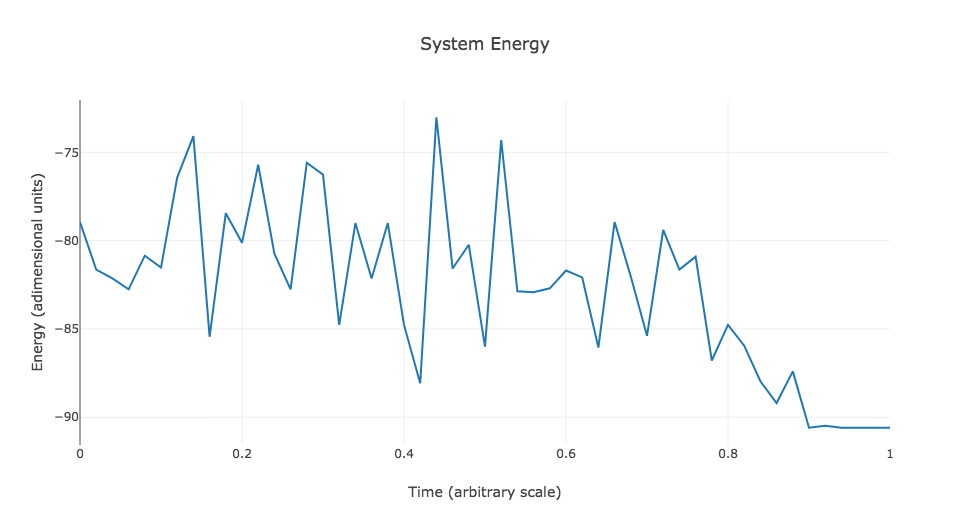
\includegraphics{SystemEnergy.png}
\caption{Plot of system energy vs. time}
\label{EnergyPlot}
\end{center}
\end{figure}
            
    \subsubsection{Distribution of developer's
choices}\label{distribution-of-developers-choices}

\begin{shaded*}
\begin{Verbatim}[commandchars=\\\{\}]
{\color{incolor}In [{\color{incolor}10}]:} \PY{n}{prefs} \PY{o}{=} \PY{n}{projPref}\PY{o}{.}\PY{n}{tolist}\PY{p}{(}\PY{p}{)}
         \PY{n}{data} \PY{o}{=} \PY{p}{[}\PY{n}{go}\PY{o}{.}\PY{n}{Bar}\PY{p}{(}
                     \PY{n}{x}\PY{o}{=}\PY{p}{[}\PY{l+s+s1}{\PYZsq{}}\PY{l+s+s1}{First Choice}\PY{l+s+s1}{\PYZsq{}}\PY{p}{,} \PY{l+s+s1}{\PYZsq{}}\PY{l+s+s1}{Second Choice}\PY{l+s+s1}{\PYZsq{}}\PY{p}{,} \PY{l+s+s1}{\PYZsq{}}\PY{l+s+s1}{Third Choice}\PY{l+s+s1}{\PYZsq{}}\PY{p}{,} \PY{l+s+s1}{\PYZsq{}}\PY{l+s+s1}{Fourth Choice}\PY{l+s+s1}{\PYZsq{}}\PY{p}{]}\PY{p}{,}
                     \PY{n}{y}\PY{o}{=}\PY{p}{[}\PY{n}{prefs}\PY{o}{.}\PY{n}{count}\PY{p}{(}\PY{l+m+mi}{1}\PY{p}{)}\PY{p}{,} \PY{n}{prefs}\PY{o}{.}\PY{n}{count}\PY{p}{(}\PY{l+m+mi}{2}\PY{p}{)}\PY{p}{,} \PY{n}{prefs}\PY{o}{.}\PY{n}{count}\PY{p}{(}\PY{l+m+mi}{3}\PY{p}{)}\PY{p}{,} \PY{n}{prefs}\PY{o}{.}\PY{n}{count}\PY{p}{(}\PY{l+m+mi}{4}\PY{p}{)}\PY{p}{]}
             \PY{p}{)}\PY{p}{]}
         \PY{n}{layout} \PY{o}{=} \PY{n+nb}{dict}\PY{p}{(}\PY{n}{title}\PY{o}{=} \PY{l+s+s1}{\PYZsq{}}\PY{l+s+s1}{Distribution of Project Allocations}\PY{l+s+s1}{\PYZsq{}}\PY{p}{,}
                      \PY{n}{yaxis} \PY{o}{=} \PY{n+nb}{dict}\PY{p}{(}\PY{n}{title}\PY{o}{=}\PY{l+s+s1}{\PYZsq{}}\PY{l+s+s1}{Developers}\PY{l+s+s1}{\PYZsq{}}\PY{p}{)}\PY{p}{)}
         \PY{n}{fig} \PY{o}{=} \PY{n+nb}{dict}\PY{p}{(}\PY{n}{data}\PY{o}{=}\PY{n}{data}\PY{p}{,} \PY{n}{layout}\PY{o}{=}\PY{n}{layout}\PY{p}{)}
         
         \PY{n}{py}\PY{o}{.}\PY{n}{iplot}\PY{p}{(}\PY{n}{fig}\PY{p}{,} \PY{n}{filename}\PY{o}{=}\PY{l+s+s1}{\PYZsq{}}\PY{l+s+s1}{basic\PYZhy{}bar}\PY{l+s+s1}{\PYZsq{}}\PY{p}{)}
\end{Verbatim}
\end{shaded*}


\begin{figure}[htbp]
\begin{center}
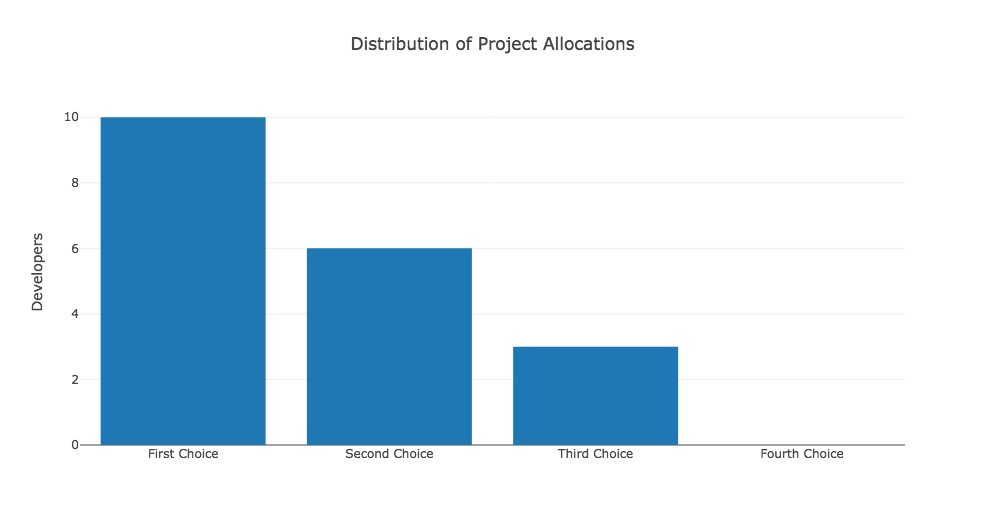
\includegraphics{Allocation.png}
\caption{Allocation Histogram}
\label{Histogram}
\end{center}
\end{figure}            

    % Add a bibliography block to the postdoc
    
    
    
    \end{document}
